% Written on Fri 22 Nov 2019 11:50:46 CET
% by Jean-Baptiste Caillau, Univ. Cote d'Azur & CNRS/Inria
\documentclass[11pt,a4paper]{article}
\usepackage{hyperref}
\usepackage{amsmath}
\usepackage{mathrsfs}
\usepackage[french]{babel}
\usepackage{graphicx}
\usepackage{wasysym}
\usepackage{tp}
\usepackage{version}
\def\N{\mathbf{N}}
\def\Z{\mathbf{Z}}
\def\Q{\mathbf{Q}}
\def\R{\mathbf{R}}
\def\C{\mathbf{C}}
\def\T{\mathbf{T}}
\def\K{\mathbf{K}}
\def\L{\mathrm{L}}
\def\H{\mathrm{H}}
\def\W{\mathrm{W}}
\def\M{\mathrm{M}}
\def\O{\mathrm{O}}
\def\CC{\mathscr{C}}
\def\Im{\mathrm{Im}}
\def\Vect{\mathrm{Vect}}
\def\Min{\mathrm{Min}}
\def\BV{\mathrm{BV}}
\def\Isom{\mathrm{Isom}}
\def\iy{\infty}
\def\d{\mathrm{d}}
\def\t{\ \!^t\!}
\def\tr{\mathrm{tr}}
\def\veps{\varepsilon}
\def\vphi{\varphi}
\def\la{\langle}
\def\ra{\rangle}
\def\noi{\noindent}
\def\cf{\emph{cf.}}
\def\ie{\emph{i.e.}}
\def\etc{\emph{etc.}}
\newcommand{\frp}[2]{\frac{\partial #1}{\partial #2}}
\newcommand{\frpp}[2]{{\partial #1}/{\partial #2}}
\newcommand{\sgn}{\mathrm{sgn}}
\renewcommand{\tilde}{\widetilde}
\renewcommand{\hat}{\widehat}
\theoremstyle{plain}
\newtheorem{thrm}{Th\'eor\`eme}[section]
\newtheorem{prpstn}{Proposition}[section]
\newtheorem{lmm}{Lemme}[section]
\newtheorem{crllr}{Corollaire}[section]
\newtheorem{dfntn}{D\'efinition}[section]
\theoremstyle{definition}
\newtheorem{rmrk}{Remarque}[section]

%\excludeversion{corr}
\includeversion{corr}

\title{Commande optimale\\Examen (CC)}
\shorttitle{Exam CC}
\numero{Exam CC}
\date{2019--2020}
\discipline{Commande optimale}
\promotion{Polytech Nice-Sophia --- MAM5 INUM}

\begin{document}
\maketitle

{\bf Dur\'ee 2H. Tous les exercices sont ind\'ependants.
Le bar\`eme pr\'e\-vi\-sion\-nel est indiqu\'e pour chaque exercice.
%Rendre sur des copies s\'epar\'ees l'exercice 1 d'une part, les exercices 2 et 3
%d'autre part.
Documents autoris\'es.}%~: une feuille de notes de cours recto-verso manuscrite.}

% Exercice 1
\begin{Exercice}[10 points]
On consid\`ere le probl\`eme de temps minimal pour
\[ \ddot{q}(t)=u(t),\quad |u(t)| \leq 1,\quad t \in [0,t_f], \]
o\`u $q$ et $u$ sont \`a valeurs dans $\R$, sous les conditions aux limites
$q(0)=q_0$, $\dot{q}(0)=\dot{q}_0$ ($q_0$ et $\dot{q}_0$ fix\'es), $\dot{q}(t_f)=0$ et
$q(t_f)$ libre.
\begin{Question}
Mettre la dynamique sous la forme $\dot{x}(t)=f(x(t),u(t))$ en posant
$x(t)=(q(t),\dot{q}(t))$, avec $f$ une fonction que l'on pr\'ecisera.
\end{Question}
\begin{corr} $\RHD$ $f(x,u)=(x_2,u)$
\end{corr}

\begin{Question} \'Ecrire le hamiltonien du probl\`eme. 
\end{Question}
\begin{corr} $\RHD$ $H(x,p,u)=p^0+p_1x_2+p_2u$
\end{corr}

\begin{Question} \'Ecrire le syst\`eme diff\'erentiel v\'erifi\'e par l'\'etat adjoint
$p=(p_1,p_2)$. \end{Question}
\begin{corr} $\RHD$ $\dot{p}_1(t)=0$, $\dot{p}_2(t)=-p_1(t)$ \end{corr}

\begin{Question} \'Ecrire les conditions de transversalit\'e. \end{Question}
\begin{corr} $\RHD$ $p_1(t_f)=0$ \end{corr}

\begin{Question} Montrer que $(p_1,p_2)$ ne s'annule jamais. \end{Question}
\begin{corr} $\RHD$
Si $p$ s'annule en un instant, il est nul partout (lin\'earit\'e de
l'\'equation adjointe en temps minimum). Mais alors $H=0$ implique aussi $p^0=0$, ce
qui est impossible. \end{corr}

\begin{Question} Montrer qu'un contr\^ole optimal doit \^etre constant. \end{Question}
\begin{corr} $\RHD$ Par maximisation, presque partout $u(t)=\sgn(p_2(t))$ si $p_2(t) \neq 0$.
Comme $p_2$ est constant
et non nul (car $p_1$ est constant et d\'ej\`a nul), on a $u$ constant \'egal \`a
$\pm 1$. \end{corr}

\begin{Question} On admet l'existence de solution, en d\'eduire l'expression du
contr\^ole en fonction de $(q_0,\dot{q}_0)$. 
\end{Question}
\begin{corr} $\RHD$ Comme $\dot{q}(t)=\dot{q}_0+ut$ avec $u=\pm 1$, pour que $\dot{q}$
puisse s'annuler en $t_f$ il faut prendre $u=-\sgn(\dot{q}_0)$. (On suppose $\dot{q}_0
\neq 0$, sinon le temps minimum est nul.)
\end{corr}

\begin{Question} En d\'eduire l'expression du temps minimal en fonction de
$(q_0,\dot{q}_0)$.
\end{Question}
\begin{corr} $\RHD$ $t_f=|\dot{q}_0|$
\end{corr}

\begin{Question} Montrer que, dans le plan $(x_1,x_2)=(q,\dot{q})$, les trajectoires
optimales sont des arcs de parabole.
\end{Question}
\begin{corr} $\RHD$ En int\'egrant la dynamique on voit que $\dot{q}^2/2-q=\text{cte}$
quand $u=1$, et que $\dot{q}^2/2+q=\text{cte}$ quand $u=-1$.
\end{corr}

\begin{Question} Donner l'allure de la synth\`ese dans le plan $(q,\dot{q})$. [Dessiner
approximativement les trajectoires temps minimales.]
\end{Question}
\begin{corr} $\RHD$ Voir Figure~\ref{fig1}.
\begin{figure}[t]
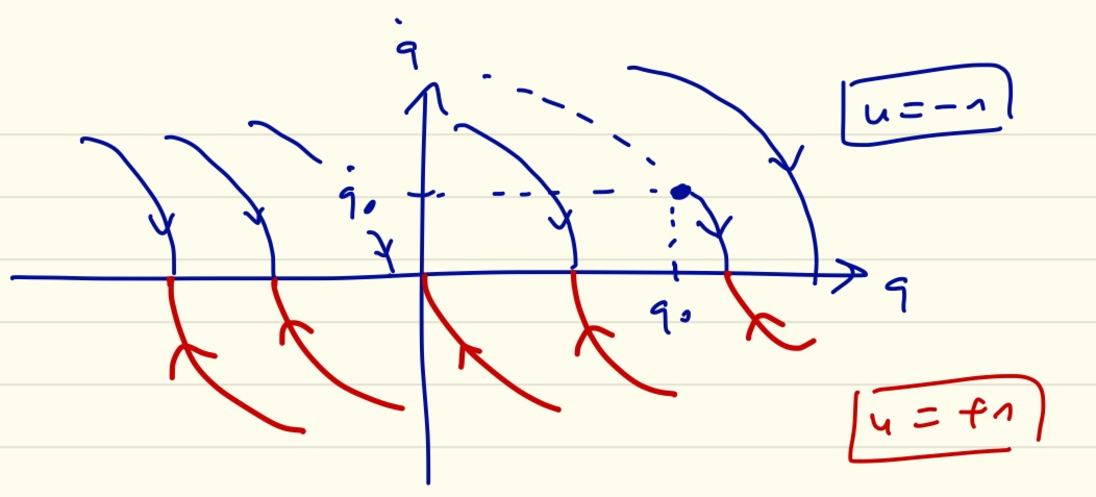
\includegraphics[width=10cm]{fig1} \centering
\caption{Trajectoires temps minimales vers la cible $\dot{q}=0$.}
\label{fig1}
\end{figure}
\end{corr}
\end{Exercice}

\newpage

% Exercice 2
\begin{Exercice}[10 points]
On consid\`ere le probl\`eme de temps minimal de Zermelo-Markov-Dubins,
\[ \dot{x}(t)=w+\cos\theta(t),\quad
   \dot{y}(t)=\sin\theta(t),\quad
   \dot{\theta}(t)=u(t),\quad t \in [0,t_f], \]
o\`u le vecteur position $(x(t),y(t))$ appartient \`a $\R^2$, l'argument de la
vitesse $\theta(t)$ \`a $\R$, et o\`u $w \in \R$ est une constante fix\'ee.
On ajoute la contrainte $|u(t)| \leq 1$ ainsi que des conditions aux limites~:
\[ (x(0),y(0),\theta(0)) = (x_0,y_0,\theta_0),\quad
   (x(t_f),y(t_f),\theta(t_f)) = (x_f,y_f,\theta_f). \]
\begin{Question} Montrer que si $|w| \geq 1$, le probl\`eme n'admet pas n\'ecessairement
de solution.
\end{Question}
\begin{corr} $\RHD$ Prenons par exemple $w=1$, $x_0=0$ et $x_f=-1$~; comme
$\dot{x}(t)$ est toujours positif, on ne pourra pas atteindre $x_f$ et l'ensemble des
contraintes est vide.
\end{corr}

On suppose d\'esormais $w \in [0,1[$, et on note $p=(p_x,p_y,p_\theta)$ l'\'etat adjoint.

\begin{Question} \'Ecrire le hamiltonien du probl\`eme.
\end{Question}
\begin{corr} $\RHD$ $H = p^0+p_x(w+\cos\theta)+p_y\sin\theta+p_\theta u$
\end{corr}

\begin{Question} \'Ecrire le syst\`eme diff\'erentiel v\'erifi\'e par l'\'etat adjoint
et montrer que $p_x$ et $p_y$ sont constants.
\end{Question}
\begin{corr} $\RHD$ On a
\[ \dot{p}_x(t)=0,\quad 
   \dot{p}_y(t)=0,\quad 
   \dot{p}_\theta(t)=p_x(t)\sin\theta(t)-p_y(t)\cos\theta(t), \]
d'o\`u la constance de $p_x$ et $p_y$.
\end{corr}

\begin{Question} Appliquer la condition de maximisation pour d\'eterminer les
contr\^oles optimaux.
\end{Question}
\begin{corr} $\RHD$ On a presque partout $u(t)=\sgn(p_\theta(t))$ si $p_\theta(t) \neq 0$.
\end{corr}

\begin{Question} En d\'eduire que, le long d'une extr\'emale optimale, on a
\[ 0 = p^0+p_x w+p_x\cos\theta(t)+p_y\sin\theta(t)+|p_\theta(t)|,\quad t \in [0,t_f]. \]
\end{Question}
\begin{corr} $\RHD$ Comme on est en temps min, $H=0$ le long d'une extr\'emale et, par
maximisation, $p_\theta(t)u(t)=|p_\theta(t)|$.
\end{corr}

On suppose d\'esormais $(p_x,p_y) \neq (0,0)$ et on pose $(p_x,p_y)=(\cos\psi,\sin\psi)$.

\begin{Question} Montrer que
\[ |p_\theta(t)|-\gamma =-\cos(\theta(t)-\psi),\quad 
   \dot{p}_\theta(t) = \sin(\theta(t)-\psi), \]
o\`u $\gamma$ est une constante que l'on pr\'ecisera.
\end{Question}
\begin{corr} $\RHD$ \'Evident d'apr\`es ce qui pr\'ec\`ede avec $\gamma=-p^0-p_x w$.
\end{corr}

\begin{Question} En d\'eduire que $(p_\theta(t),\dot{p}_\theta(t))$ appartient \`a un
ensemble que l'on dessinera pour $\gamma > 1$.
\end{Question}
\begin{corr} $\RHD$ Il s'agit de la r\'eunion de deux cercles (\'eventuellement
tronqu\'es selon la position des centres) de rayon $1$ et de centres $\pm \gamma$.
Quand $\gamma > 1$, les deux cercles sont disjoints, chacun dans un demi-plan, voir
Figure~\ref{fig2}.
\begin{figure}[t]
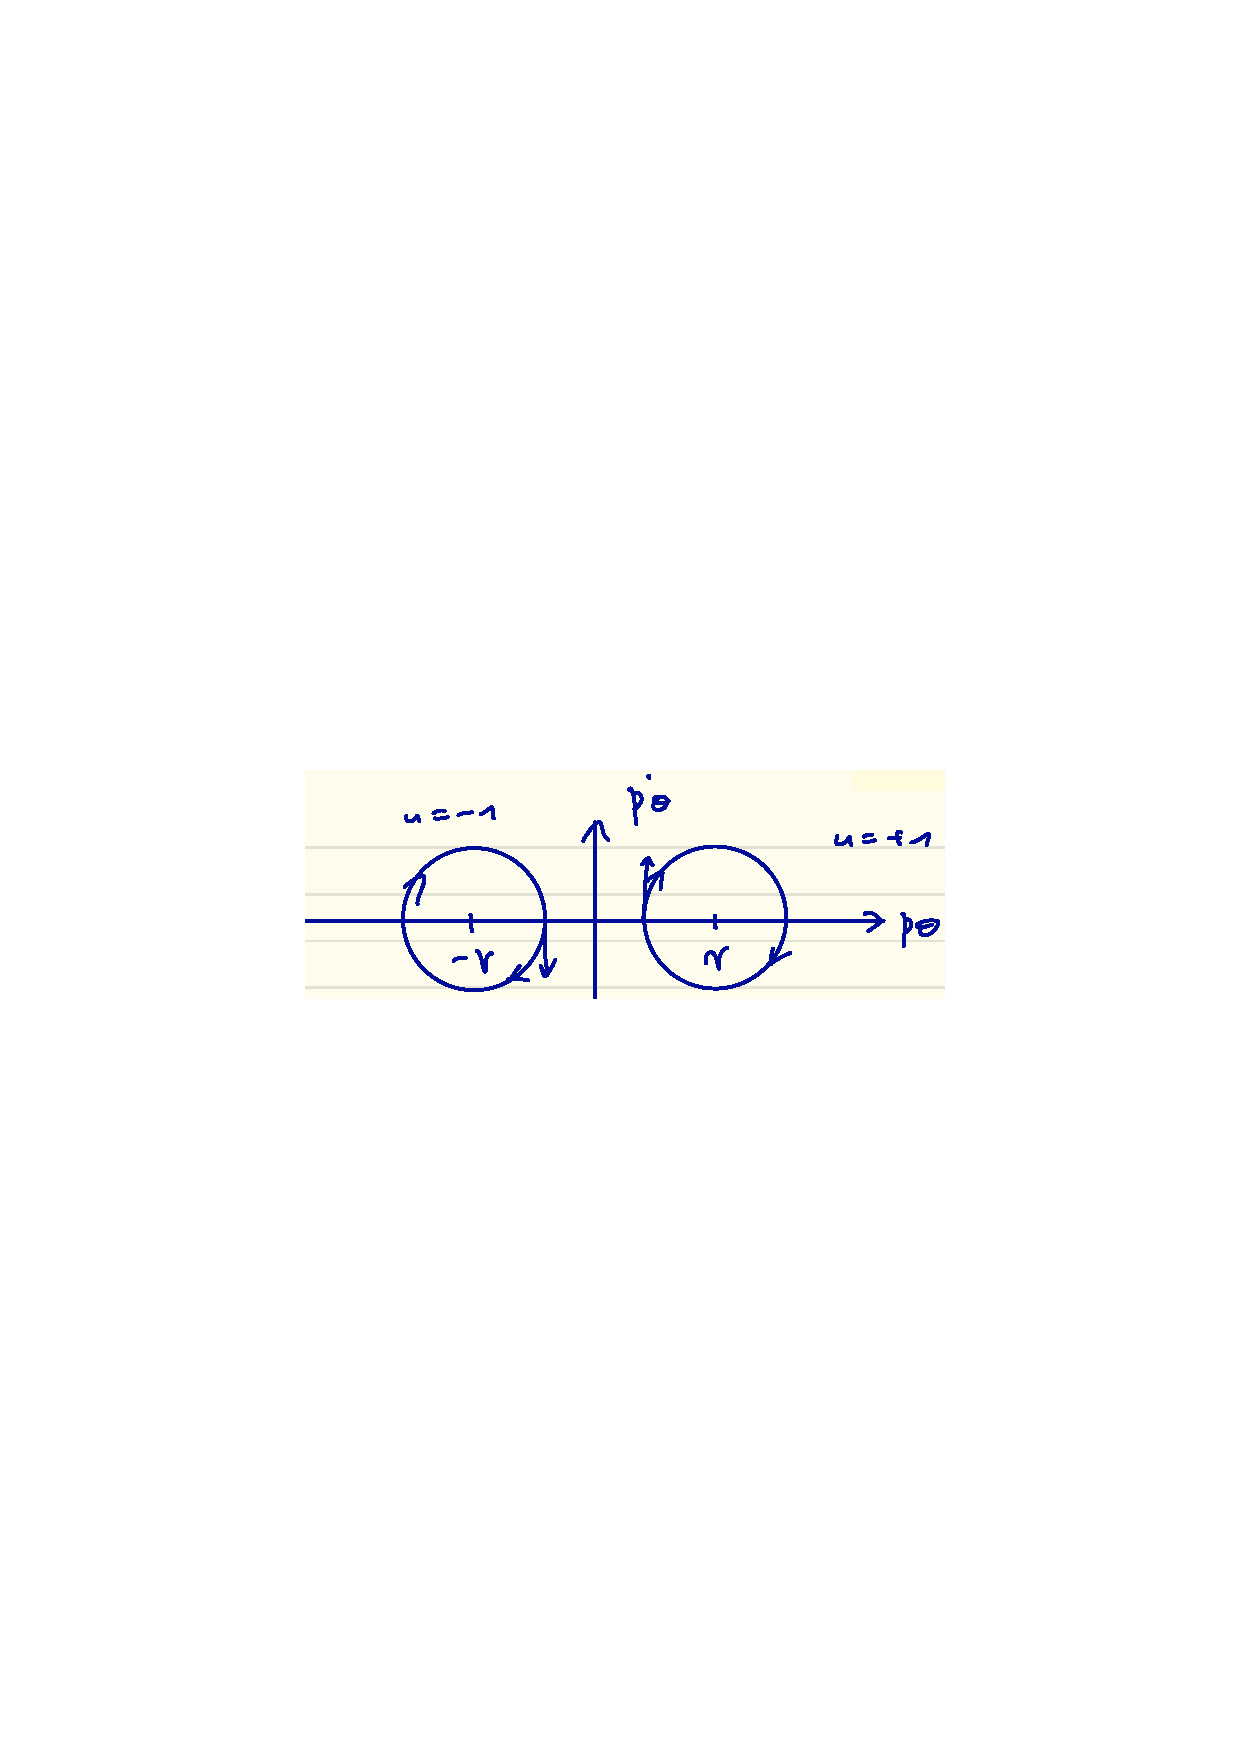
\includegraphics[width=10cm]{fig2} \centering
\caption{Extr\'emales dans le plan $(p_\theta,\dot{p}_\theta)$.}
\label{fig2}
\end{figure}
\end{corr}

\begin{Question} Dans le cas $\gamma > 1$, montrer que le contr\^ole est constant,
\'egal \`a $\pm 1$.
\end{Question}
\begin{corr} $\RHD$ Les deux cercles \'etant disjoints, et $(p_\theta,\dot{p}_\theta)$
\'etant continues (au vu de l'\'equation diff\'erentielle v\'erifi\'ee par
$p_\theta$), on est soit sur le cercle dans $p_\theta<0$ (auquel cas $u=-1$), soit sur
le cercle dans $p_\theta>0$ (auquel cas $u=1$).
\end{corr}

\begin{Question} Dans le cas o\`u le contr\^ole est constant \'egal \`a $+1$, donner
l'expression de $x(t)$, $y(t)$ et $\theta(t)$.
\end{Question}
\begin{corr} $\RHD$ $\theta(t)=\theta_0+t$, $x(t)=x_0+wt+\sin\theta(t)-\sin\theta_0$,
$y(t)=y_0-\cos\theta(t)+\cos\theta_0$
\end{corr}

\end{Exercice}

\end{document}

\begin{Exercice}
\begin{Question}
\end{Question}
\begin{corr} $\RHD$
\end{corr}
\end{Exercice}
